\begin{table*}[t]
\centering\footnotesize
\begin{tabular}{llrrrrrr}
\toprule
Task & $T$ & Uncalibrated & Local & Graph & Mixed & Output bias & Shuffled targets \\
\midrule
MNIST & 1 & 71.99 $\pm$ 3.04 & 79.19 $\pm$ 1.67 & 79.09 $\pm$ 1.61 & 79.09 $\pm$ 1.70 & 72.15 $\pm$ 2.93 & 38.44 $\pm$ 2.83 \\
MNIST & 2 & 91.00 $\pm$ 0.29 & 91.33 $\pm$ 0.50 & 91.21 $\pm$ 0.48 & 91.27 $\pm$ 0.36 & 91.02 $\pm$ 0.38 & 50.79 $\pm$ 6.92 \\
MNIST & 4 & 92.13 $\pm$ 0.20 & 92.14 $\pm$ 0.22 & 92.18 $\pm$ 0.18 & 92.15 $\pm$ 0.17 & 92.12 $\pm$ 0.20 & 59.65 $\pm$ 9.99 \\
MNIST & 8 & 92.20 $\pm$ 0.19 & 92.19 $\pm$ 0.18 & 92.21 $\pm$ 0.19 & 92.22 $\pm$ 0.18 & 92.20 $\pm$ 0.19 & 72.57 $\pm$ 2.66 \\
\midrule
CIFAR10 & 1 & 47.59 $\pm$ 1.26 & 50.60 $\pm$ 0.82 & 50.33 $\pm$ 1.17 & 50.19 $\pm$ 1.26 & 47.69 $\pm$ 1.28 & 24.39 $\pm$ 2.22 \\
CIFAR10 & 2 & 55.63 $\pm$ 0.87 & 55.37 $\pm$ 0.67 & 55.81 $\pm$ 0.75 & 55.55 $\pm$ 0.85 & 55.69 $\pm$ 0.79 & 29.12 $\pm$ 1.24 \\
CIFAR10 & 4 & 56.19 $\pm$ 0.72 & 56.13 $\pm$ 0.72 & 56.21 $\pm$ 0.77 & 56.24 $\pm$ 0.75 & 56.19 $\pm$ 0.73 & 37.81 $\pm$ 2.98 \\
CIFAR10 & 8 & 56.15 $\pm$ 0.72 & 56.15 $\pm$ 0.71 & 56.13 $\pm$ 0.65 & 56.15 $\pm$ 0.71 & 56.15 $\pm$ 0.70 & 47.30 $\pm$ 3.95 \\
\bottomrule
\end{tabular}
\caption{Full official validation accuracy (percent), mean $\pm$ sample SD across three teacher seeds. Each seed uses the same 5,000 graphs; calibration uses 512 training graphs and 64 updates. All six frozen conditions are retained.}
\label{tab:validation}
\end{table*}

\begin{table*}[t]
\centering\small
\begin{tabular}{llrrrrr}
\toprule
Task & $T$ & Seed 41 & Seed 42 & Seed 43 & Mean $\pm$ SD & $t$-95\% interval \\
\midrule
MNIST & 1 & +0.25 & -0.27 & -0.36 & -0.13 $\pm$ 0.32 & [-0.93, +0.68] \\
MNIST & 2 & +0.02 & -0.29 & -0.09 & -0.12 $\pm$ 0.16 & [-0.51, +0.27] \\
CIFAR10 & 1 & -0.85 & -0.98 & +0.60 & -0.41 $\pm$ 0.88 & [-2.59, +1.77] \\
CIFAR10 & 2 & +0.25 & +0.13 & +0.60 & 0.33 $\pm$ 0.24 & [-0.28, +0.93] \\
\bottomrule
\end{tabular}
\caption{Graph-minus-local accuracy differences (percentage points) on the 4,488 validation graphs outside the current screen. Intervals use three seed-level differences and two degrees of freedom; they remain descriptive on historically exposed validation data.}
\label{tab:paired}
\end{table*}

\begin{table*}[t]
\centering\footnotesize
\begin{tabular}{llrrrrrr}
\toprule
Task & $T$ & Uncalibrated & Local & Graph & Mixed & Output bias & Shuffled targets \\
\midrule
MNIST & 1 & 71.44 $\pm$ 2.80 & 78.50 $\pm$ 2.10 & 78.70 $\pm$ 2.19 & 78.95 $\pm$ 2.08 & 71.61 $\pm$ 2.80 & 39.81 $\pm$ 1.45 \\
MNIST & 2 & 90.16 $\pm$ 0.49 & 90.08 $\pm$ 0.26 & 90.26 $\pm$ 0.35 & 90.19 $\pm$ 0.44 & 90.17 $\pm$ 0.51 & 52.22 $\pm$ 6.54 \\
MNIST & 4 & 91.04 $\pm$ 0.26 & 91.00 $\pm$ 0.28 & 91.01 $\pm$ 0.28 & 91.01 $\pm$ 0.24 & 91.05 $\pm$ 0.26 & 60.56 $\pm$ 8.79 \\
MNIST & 8 & 91.01 $\pm$ 0.26 & 91.02 $\pm$ 0.25 & 91.03 $\pm$ 0.27 & 91.03 $\pm$ 0.29 & 91.01 $\pm$ 0.26 & 72.40 $\pm$ 2.36 \\
\midrule
CIFAR10 & 1 & 46.80 $\pm$ 1.22 & 49.92 $\pm$ 0.14 & 49.75 $\pm$ 0.68 & 49.72 $\pm$ 0.32 & 47.00 $\pm$ 1.18 & 24.34 $\pm$ 2.55 \\
CIFAR10 & 2 & 54.07 $\pm$ 0.24 & 54.18 $\pm$ 0.14 & 54.37 $\pm$ 0.26 & 54.42 $\pm$ 0.25 & 54.08 $\pm$ 0.28 & 28.45 $\pm$ 0.41 \\
CIFAR10 & 4 & 54.91 $\pm$ 0.06 & 54.96 $\pm$ 0.09 & 54.97 $\pm$ 0.05 & 54.90 $\pm$ 0.05 & 54.91 $\pm$ 0.06 & 36.76 $\pm$ 3.42 \\
CIFAR10 & 8 & 54.96 $\pm$ 0.04 & 54.95 $\pm$ 0.08 & 54.97 $\pm$ 0.11 & 54.99 $\pm$ 0.08 & 54.96 $\pm$ 0.03 & 46.32 $\pm$ 3.62 \\
\bottomrule
\end{tabular}
\caption{Once-frozen full official test endpoints (10,000 historically exposed graphs per task), mean $\pm$ sample SD over three teacher seeds. No updates or model selection occur in this evaluation.}
\label{tab:test}
\end{table*}


\subsection{Fidelity and objective choice}

Tables~\ref{tab:validation}--\ref{tab:test} retain all six conditions. At $T=1$, local reconstruction improves mean test accuracy from 71.44\% to 78.50\% on MNIST and from 46.80\% to 49.92\% on CIFAR10.

The additional effect of the graph objective is much smaller. Graph-minus-local test differences at $T=1/2$ are +0.20/+0.18 percentage points on MNIST and -0.18/+0.19 on CIFAR10.

On full validation, the corresponding means are $-0.10/-0.13$ and $-0.27/+0.43$ points. Excluding the 512 current-screen graphs reduces the CIFAR10 $T=2$ mean to $+0.33$ points; its three-seed interval spans zero. The fixed mixture also lacks a consistent advantage across tasks and splits. Its strongest short-prefix test gain over local calibration is $+0.45$ points on MNIST $T=1$, compared with $-0.10$ on full validation. These outcomes fall short of the screening criterion of a stable, practically meaningful gain in multiple settings.

By $T=4/8$, uncalibrated conversion is already close to teacher accuracy. The small remaining changes should be read alongside teacher agreement and reconstruction error rather than ranked as reliable improvements.

\begin{figure*}[t]\centering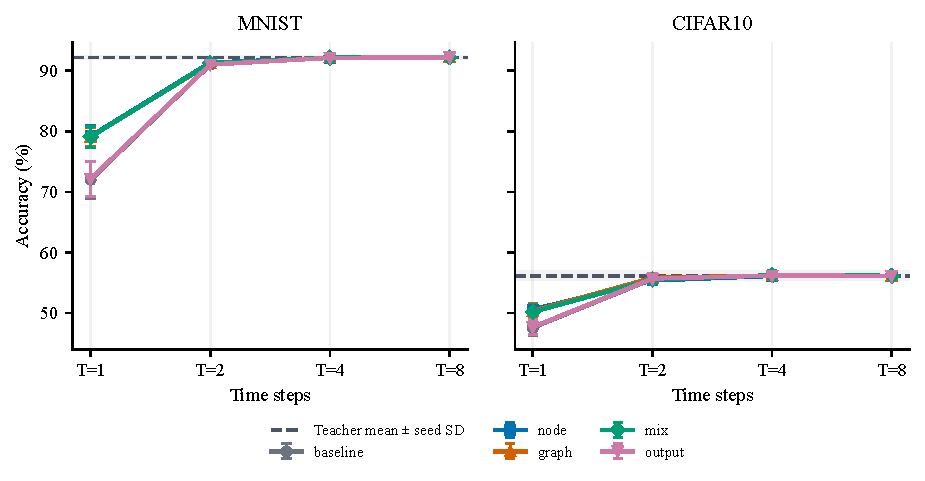
\includegraphics[width=\textwidth]{../figures/accuracy_curves.pdf}\caption{Full validation fidelity across three teacher seeds. Error bars are sample SD. Teacher reference bands use the corresponding validation mean and SD. All optimized conditions use the frozen smaller-step configuration.}\label{fig:accuracy}\end{figure*}

\begin{figure*}[t]\centering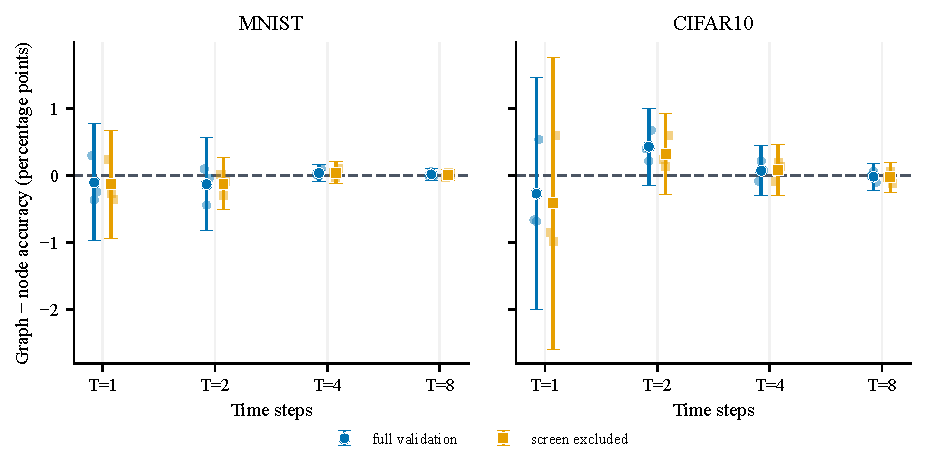
\includegraphics[width=\textwidth]{../figures/paired_objective.pdf}\caption{Graph-minus-local accuracy differences on full validation and the 4,488 examples outside the current screen. Small markers show each teacher seed; intervals use the paired three-seed $t$ distribution with two degrees of freedom. Both subsets have historical exposure.}\label{fig:paired}\end{figure*}

\subsection{Error association and conditional location}

On the screen-excluded examples, graph-logit MSE is more correlated with flips than the four-node-site error aggregate in all twelve task/seed/low-prefix cells. Including the two MLP sites raises the local proxy correlation, while the output proxy remains stronger on average. Teacher margin is more predictive still: mean flip-ranking AUC for negative margin is 0.77/0.96 on MNIST $T=1/2$ and 0.73/0.90 on CIFAR10, compared with 0.67/0.61 and 0.59/0.59 for graph-logit MSE. These are marginal associations on the same graphs.

The ideal interventions identify a different question: which quantizers conditionally cause the observed discrepancy? At $T=1$, restoring all four node sites closes 80.4\%/45.2\% of the MNIST/CIFAR10 disagreement gaps, versus 8.8\%/14.9\% when restoring only the two readout sites.

The first node site alone closes about 54.1\%/23.5\%, and gives the largest individual-site accuracy recovery in both tasks. This supports an important upstream quantization effect in this architecture rather than a dominant readout-only explanation. At $T=2$, node and readout group effects are closer on CIFAR10. Restoring all sites reproduces the folded teacher exactly in these runs. These continuous-valued interventions restore different numbers of sites and can interact; their effects are conditional rather than additive.

\begin{table*}[t]\centering\footnotesize
\begin{tabular}{llrrrrr}\toprule
Task & $T$ & Baseline & First node (1) & All node (4) & Readout (2) & All sites (6) \\ \midrule
MNIST & 1 & 71.99 $\pm$ 3.04 & 84.88 $\pm$ 1.50 & 90.14 $\pm$ 0.25 & 74.17 $\pm$ 2.67 & 92.18 $\pm$ 0.20 \\
MNIST & 2 & 91.00 $\pm$ 0.29 & 91.71 $\pm$ 0.23 & 91.95 $\pm$ 0.21 & 91.49 $\pm$ 0.44 & 92.18 $\pm$ 0.20 \\
CIFAR10 & 1 & 47.59 $\pm$ 1.26 & 51.12 $\pm$ 1.14 & 52.97 $\pm$ 0.33 & 50.19 $\pm$ 1.25 & 56.15 $\pm$ 0.69 \\
CIFAR10 & 2 & 55.63 $\pm$ 0.87 & 55.78 $\pm$ 0.90 & 55.95 $\pm$ 0.75 & 55.87 $\pm$ 0.74 & 56.15 $\pm$ 0.69 \\
\bottomrule\end{tabular}
\caption{Ideal-site validation accuracy (percent), mean $\pm$ sample SD over three teachers. Parentheses give numbers of restored nonlinearities. These are continuous-valued diagnostic interventions with zero fitted offsets, not deployable spiking competitors or budget-matched algorithms. All six ideal sites recover the teacher.}\label{tab:ideal}\end{table*}


\subsection{Calibration and software cost}

Local and graph conditions share their inference computation and differ only in fitted initial states. Their measured times are nearly coincident (Figure~\ref{fig:latency}). The one-tick baseline core averages 0.366/0.493 ms per graph on MNIST/CIFAR10, versus 0.152/0.157 for the teachers.

The conversion core at $T=8$ averages 2.407/3.451 ms per graph. These are means of three per-seed batch medians divided by 32, with raw repeated timings retained. The diagnostic core returns site activations as well as logits, so these ratios describe its actual implementation rather than a best-achievable backend bound.

The three-seed mean times of the 64-update local/graph calibration loops are about 1.1--2.6 seconds per low-prefix condition, excluding shared data loading, checks and target preparation. Dense graph projections and edge reductions run at every tick regardless of zero-event counts. The arithmetic ledger records those projections and reductions as a partial lower bound; it excludes neuron-state arithmetic and memory traffic and therefore cannot serve as a complete energy estimate. Physical energy remains unmeasured.

\begin{figure*}[p]\centering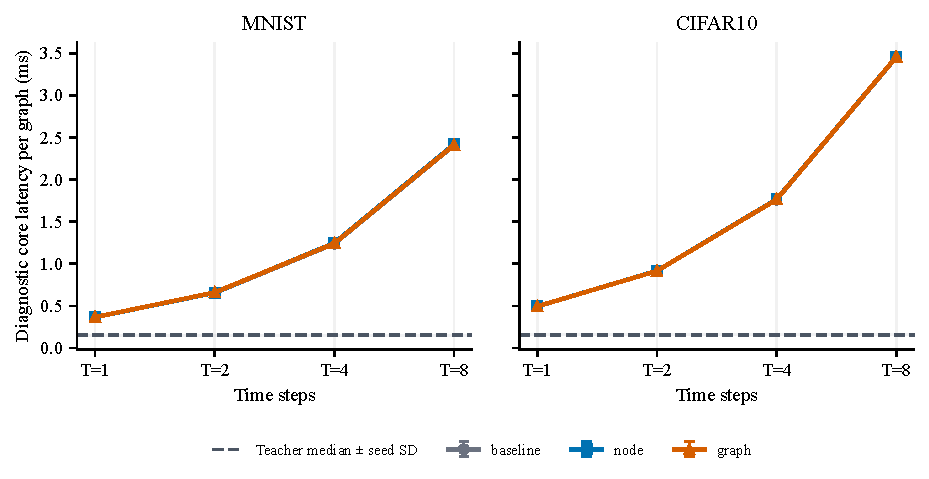
\includegraphics[width=\textwidth]{../figures/latency.pdf}\caption{Synchronized diagnostic-core runtime on a fixed cached batch of 32 graphs. Points summarize three teacher-seed medians; error bars show their sample SD. Each condition has ten warmups and thirty randomized interleaved repeats. Data transfer is excluded.}\label{fig:latency}\end{figure*}

\subsection{Failure conditions}

The initial $10^{-2}$ step size increased MNIST $T=2$ hard training logit MSE from 0.685 to 0.966; the single smaller-step correction improved optimization but did not produce a stable graph-objective advantage. Shuffling targets substantially degrades fidelity at every tested prefix, establishing target-correspondence sensitivity. That result is compatible with ordinary distillation and does not identify a topology-specific mechanism. The unchanged original screen, all per-seed endpoints and individual-site interventions accompany the summaries.

\begin{table*}[p]\centering\footnotesize
\begin{tabular}{llrrrrrrrr}\toprule
Task & Seed & $T$ & ANN & Uncalibrated & Local & Graph & Mixed & Output & Shuffled \\ \midrule
MNIST & 41 & 1 & 90.94 & 74.46 & 78.48 & 78.68 & 78.88 & 74.62 & 39.10 \\
MNIST & 41 & 2 & 90.94 & 90.16 & 89.96 & 90.13 & 90.26 & 90.10 & 53.74 \\
MNIST & 41 & 4 & 90.94 & 90.94 & 90.86 & 90.79 & 90.97 & 90.94 & 52.57 \\
MNIST & 41 & 8 & 90.94 & 90.93 & 90.95 & 90.93 & 90.93 & 90.93 & 72.82 \\
\addlinespace[2pt]
MNIST & 42 & 1 & 91.32 & 70.92 & 80.61 & 80.90 & 81.06 & 71.14 & 41.47 \\
MNIST & 42 & 2 & 91.32 & 90.64 & 90.38 & 90.65 & 90.59 & 90.71 & 57.87 \\
MNIST & 42 & 4 & 91.32 & 91.33 & 91.33 & 91.33 & 91.27 & 91.34 & 69.98 \\
MNIST & 42 & 8 & 91.32 & 91.30 & 91.30 & 91.34 & 91.36 & 91.30 & 74.52 \\
\addlinespace[2pt]
MNIST & 43 & 1 & 90.81 & 68.93 & 76.41 & 76.53 & 76.90 & 69.07 & 38.85 \\
MNIST & 43 & 2 & 90.81 & 89.67 & 89.90 & 89.99 & 89.72 & 89.70 & 45.05 \\
MNIST & 43 & 4 & 90.81 & 90.85 & 90.82 & 90.91 & 90.80 & 90.86 & 59.14 \\
MNIST & 43 & 8 & 90.81 & 90.81 & 90.82 & 90.82 & 90.80 & 90.81 & 69.85 \\
\addlinespace[2pt]
CIFAR10 & 41 & 1 & 54.87 & 45.48 & 49.87 & 49.13 & 49.46 & 45.75 & 22.84 \\
CIFAR10 & 41 & 2 & 54.87 & 53.87 & 54.27 & 54.13 & 54.17 & 53.88 & 28.09 \\
CIFAR10 & 41 & 4 & 54.87 & 54.88 & 54.86 & 54.92 & 54.85 & 54.89 & 38.92 \\
CIFAR10 & 41 & 8 & 54.87 & 54.93 & 54.88 & 54.86 & 54.92 & 54.93 & 48.74 \\
\addlinespace[2pt]
CIFAR10 & 42 & 1 & 54.94 & 47.90 & 49.82 & 50.48 & 50.08 & 48.10 & 22.89 \\
CIFAR10 & 42 & 2 & 54.94 & 54.00 & 54.01 & 54.33 & 54.67 & 53.97 & 28.89 \\
CIFAR10 & 42 & 4 & 54.94 & 54.86 & 54.99 & 54.96 & 54.95 & 54.87 & 38.54 \\
CIFAR10 & 42 & 8 & 54.94 & 54.95 & 54.93 & 54.97 & 54.97 & 54.95 & 48.05 \\
\addlinespace[2pt]
CIFAR10 & 43 & 1 & 55.01 & 47.01 & 50.08 & 49.63 & 49.62 & 47.14 & 27.29 \\
CIFAR10 & 43 & 2 & 55.01 & 54.34 & 54.25 & 54.65 & 54.43 & 54.40 & 28.37 \\
CIFAR10 & 43 & 4 & 55.01 & 54.98 & 55.03 & 55.02 & 54.91 & 54.98 & 32.81 \\
CIFAR10 & 43 & 8 & 55.01 & 55.00 & 55.04 & 55.08 & 55.08 & 54.99 & 42.16 \\
\addlinespace[2pt]
\bottomrule\end{tabular}
\caption{Individual frozen test accuracies (percent) underlying Table~\ref{tab:test}. Each row uses the same teacher checkpoint and all 10,000 official test graphs, with no fitting at test time. The official test split has historical exposure.}\label{tab:individual}\end{table*}

